\documentclass{article}
\usepackage[UTF8]{ctex}
\usepackage{geometry}
\usepackage{makecell}
\usepackage{amsmath}
\usepackage{graphicx}
\usepackage{subcaption}

\geometry{a4paper,scale=0.75}

\title{\heiti 实验二十一\ 观察光的偏振现象}
\author{\kaishu 田睿轩\ 物理学院\ 1900011602}
\date{2020年11月26日}
\newcommand{\degree}{^\circ}
%大写罗马字母:\uppercase\expandafter{\romannumeral1}
%小写罗马字母:\romannumeral1


\begin{document}
    \maketitle

    \section{实验现象的描述与解释}
    \subsection{用偏振光镜验证布儒斯特定律}
    使用如下图所示的偏振光镜验证布儒斯特定律。
    
    \begin{center}
        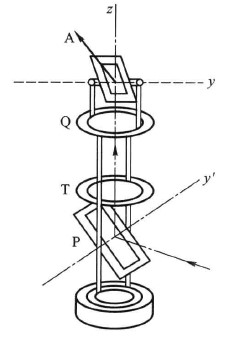
\includegraphics[width=0.3\textwidth]{偏振光镜.jpg}
    \end{center}

    调节激光器的,使其以$24\degree$的仰角发出激光;再调节玻璃片P的仰角,使其与竖直方向成$33\degree$。这样,
    激光能以$57\degree$这一接近布儒斯特角的角度入射,同时反射光也能竖直向上射出。

    \begin{enumerate}
        \item [(1)]
        先使A//P,绕$z$轴旋转A,观察反射光强度的变化:
        
        设A//P时,旋转角度为$0\degree$。则当旋转角度从$0\degree$增加到$90\degree$的过程中,反射光强度逐渐减小,
        $90\degree$时反射光强度几乎为0;而从$90\degree$旋转到$180\degree$的过程中,反射光强度逐渐增大,
        旋转角度为$180\degree$时与$0\degree$时为光强最大时。

        该现象的出现是因为当光以布儒斯特角入射镜面P时,反射光只有S方向的偏振光(以偏振光镜架的坐标系来说,反射光的偏振方向沿$y'$方向),
        上方的玻璃片堆A因为与玻璃片P平行且绕$z$轴旋转过程中入射角不变,光线也以布儒斯特角入射,
        所以也只会反射S方向的偏振光。当旋转角度为$0\degree$时,A玻璃片堆的入射光全部为相对于A的S方向偏振光,
        所以反射光强度最强;而旋转角度为$90\degree$,A玻璃片堆的入射光全部为相对于片堆的P方向偏振光,因此反射光强度为0。
        在从$0\degree$旋转到$90\degree$的过程中,A堆反射的是沿$y'$方向的偏振光在A的S方向上的投影,因此光强呈单调递减趋势。

        不过由于实验中装置的调节精度的限制,无法使光以真正的布儒斯特角入射,而且激光的偏振性也无法保证为完全的线偏振光,
        所以实验现象只是近似地满足理论预期。如实验中观察到A与P相互正交时反射光其实不为0,但光强的相对变化还是非常符合理论的预期的。

        \item [(2)]
        A//P,绕$z$轴旋转A,观察透射光强度的变化:

        旋转角度为$0\degree$时,透射光强度最小,但不为0;旋转角度为$0\degree$时,透射光强度最大。从$0\degree$到$90\degree$的过程中透射光
        强度逐渐增大。

        该现象的出现是因为光经过玻璃片堆之后的透射光S偏振方向的光强小于P方向的光强,且随着玻璃片数目的增加,S光光强
        所占比例越小,当玻璃片数目足够多时,透射光几乎都为P光。在本实验中,旋转角度为$0\degree$时,A玻璃片堆的入射光全部为相对于A的S方向偏振光,
        所以透射率很低,而旋转角度为$90\degree$时,入射光全为P光,几乎都能透过,所以透射率接近1,透射光强度最大。

        或者也可以从另一角度理解该现象,根据能量守恒,反射率和透射率加和为1,反射光强度最大时即为透射光强度最小时,反射光强度最小时即为透射光强度最大时。

        \item [(3)]
        将A绕$z$轴转至反射光消光的位置,然后将A绕y轴转动,观察反射光强度的变化:

        当玻璃片堆A与竖直方向夹角为$33\degree$,也即光以布儒斯特角入射时,反射光强度最小(几乎为0),当入射角分别向$0\degree$和$90\degree$
        变化时,反射光强度均单调增加。

        当玻璃片堆处在该位置时,入射光均为P光,根据布儒斯特定律,P光的透射率随着入射角的增大,先减小后增大,在布儒斯特角处取到最小值0。
        所以将A绕y轴向两个方向旋转,反射光强度会增加。

        \item [(4)]
        将A绕$z$轴转至反射光消光的位置,然后将A绕y轴转动,观察透射光强度的变化:

        转动过程中,透射光强度无明显变化。

        该旋转角度下,入射光全部为P光,玻璃片堆对P光的透过率也遵循先增大后减小,在布儒斯特角处取最大值的变化情况,
        但在入射角不是很接近$90\degree$的情况下,透过率的最小值和最大值相差不大,所以这个最小值和最大值的比例非常接近1,
        而人眼又是一个非线性响应(对数相应),所以人眼便几乎察觉不出光强的变化。与之相对的是,在前面所做的1、2、3项实验中,
        光强变化情况分别是:从某一值变到0,从一接近0的值变到1,和从某一直变到0在变到另一值,光强最大最小值的比值是远大于1的。
        所以另外3个实验都能观察到明显现象,而该实验观察不到光强的明显变化。

        \item [(5)]
        利用已知透光方向的偏振片确定P的反射光是否为线偏振光:

        将偏振镜片放在置物台T上,旋转偏振镜片,通过观察光线经过偏振片后找到A玻璃堆上的光斑的亮暗来确定其亮度。
        在偏振片旋转$360\degree$的过程中,光斑出现两次极强和两次消光,极强和消光之间偏振片的旋转角度为$90\degree$。
        这说明经过P反射后产生的光线确实为线偏振光。
    \end{enumerate}

    \subsection{观察双折射现象}
    实验中使用的方解石是一种双折射晶体,而且是单轴晶体。光线经过其中会发生双折射产生寻常光(o光)和非寻常光(e)光。
    实验中,将两种不同的方解石晶体置于小孔光源上,观察现象。

    \begin{itemize}
        \item [(1)]
        小孔上放方解石\uppercase\expandafter{\romannumeral1},观察现象

        可以透过方解石看到两个小孔的像,转动方解石,两个小孔的连线始终平行于平行六面体的对角线。

        该现象的产生是因为小孔光源经过方解石发生双折射,形成两道光进而形成两个像,这两个像的连线平行于光轴。

        \item [(2)]
        小孔上放方解石\uppercase\expandafter{\romannumeral2},观察现象

        将方解石\uppercase\expandafter{\romannumeral2}的磨面压在小孔上,透过另一磨面观察,此时只能看到
        小孔光源的一个像,且旋转方解石,像的位置基本不发生变化。

        该方解石的磨面恰好为垂直于方解石光轴的两平面,因此小孔发出的光以平行于光轴的方向入射,因此不会分成寻常光
        和非寻常光,所以在另一磨面上观察,只会看到一个像。

        \item [(3)]
        利用一透光方向已知的偏振片,判断寻常光与非寻常光电矢量的振动方向

        将方解石\uppercase\expandafter{\romannumeral1}放在光源上,并在其上方通过偏振片观察两个像。
        旋转偏振片,两个光斑的亮度发生周期性变化。对于某一个像,在偏振片旋转$360\degree$的过程中,像的亮度出现两次极强和两次消光,
        极强和消光的间隔为$90\degree$。而对于两个像,其中一个像消光时另一个像正好亮度最大,反之亦然。

        经方解石双折射产生的寻常光和非寻常光均为线偏振光,且偏振方向互相正交,因此会出现上述现象。
    \end{itemize}

    \subsubsection{观察线偏振光透过$\frac{\lambda}{2}$片后的现象}
    $\frac{\lambda}{2}$片是波晶片的一种,它能使入射光线经过波晶片后出射时加上$\pi$的相位差。
    本实验中探究线偏振光透过$\frac{\lambda}{2}$片后的现象的光路图如下图所示:
    
    \begin{center}
        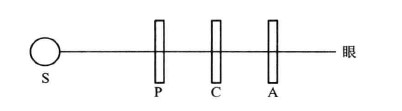
\includegraphics[width=0.6\textwidth]{波晶片.jpg}
    \end{center}

    \begin{itemize}
        \item [(1)]
        了解偏振片P,A的作用:

        在观察着和光源S之间放入偏振片P,旋转P,透射光强度无显著变化。这是因为光源发出的光为自然光,具有各向同性,
        不同线偏振方向上强度相等。

        放上检偏器A,转动A,透射光强度发生亮暗变化,最亮和消光间隔$90\degree$交替出现,转动$360\degree$过程中,
        出现两次消光和两次光强最大。这是因为光源发出的光经过偏振片P后透射光为线偏振光,该光中只有在A的偏振方向上的
        分量可以透过偏振片A,所以随着A的旋转,透射光发生周期性变化。当A的偏振方向与P的偏振方向平行,透射光强度最大;
        当两者正交,出现消光。

        \item [(2)]
        P、A正交,在它们中间插入$\frac{\lambda}{2}$片,将$\frac{\lambda}{2}$片转动$360\degree$并观察现象:

        转动$\frac{\lambda}{2}$片一周的过程中一共出现四次消光,每两次间隔$90\degree$。$\frac{\lambda}{2}$片
        会使透过的光的偏振方向发生改变,出射光和入射光的振动方向关于波晶片的光轴对称。实验中,当波晶片的光轴与P的偏振方向平行
        或夹角为$90\degree$时($\frac{\lambda}{2}$片转动$360\degree$过程中总共会有四个位置满足上述条件),
        出射光的偏振方向均与入射光的偏振方向平行,由于PA正交,因此在这四个位置透过P、C、A观察会出现消光。

        \item [(3)]
        把$\frac{\lambda}{2}$片转动任意角度,破坏消光现象,再将A转动$360\degree$,观察出现消光的次数:

        转动过程中能看到两次消光,间隔$180\degree$。偏振片P的出射光经过$\frac{\lambda}{2}$片偏振方向发生了改变,
        但仍然是线偏振光,因此用偏振片A进行观察,当A的偏振方向和C的出射光线偏振方向正交时,出现消光。A旋转$360\degree$
        过程中总共会出现两次与C出射光线正交的位置,间隔$180\degree$,因此会有两次消光。

        \item [(4)]
        PA正交,中间插入$\frac{\lambda}{2}$片,转动使之消光(此时$\frac{\lambda}{2}$片的e轴或o轴平行于P的透光方向),
        以此时P和$\frac{\lambda}{2}$片位置对应角度为$0\degree$,
        保持$\frac{\lambda}{2}$片不动,将P转过不同角度$\theta$,再将A反方向旋转至消光位置,记录A转的角度$\theta '$

        \begin{center}
            \begin{tabular}{|c|c|c|}
                \hline
                $\theta$ & $\theta '$ & 线偏振光经$\frac{\lambda}{2}$片后振动方向转过的角度 \\
                \hline
                $0\degree$ & $0\degree$ & $0\degree$ \\
                \hline
                $15\degree$ & $15\degree$ & $30\degree$ \\
                \hline
                $30\degree$ & $30\degree$ & $60\degree$ \\
                \hline
                $45\degree$ & $45\degree$ & $90\degree$ \\
                \hline
                $60\degree$ & $60\degree$ & $120\degree$ \\
                \hline
                $75\degree$ & $75\degree$ & $150\degree$ \\
                \hline
                $90\degree$ & $90\degree$ & $180\degree$ \\
                \hline
            \end{tabular}
        \end{center}
        
        $\frac{\lambda}{2}$片会使使入射光和出射光的振动方向关于波晶片光轴对称,因此,若P转动了一定角度,
        其透射光经过$\frac{\lambda}{2}$片后应反方向转过了相同角度,A偏振片也要沿该方向转过相同角度才能消光。
    \end{itemize}

    \subsection{用$\frac{\lambda}{4}$片产生椭圆偏振光}
    实验装置与上实验相同。
    取下$\frac{\lambda}{2}$片,仍使P、A正交,中间插入$\frac{\lambda}{4}$片,旋转使之消光,
    此时$\frac{\lambda}{4}$片的e轴或o轴平行于P的透光方向,\textbf{为了方便起见,我们不妨设e轴平行于P的透光方向。}
    $\frac{\lambda}{4}$片会使入射光在o轴方向上的投影加上$\frac{\pi}{2}$的相位,因此线偏振光透过后如果原偏振方向不与光轴平行,
    可以变为椭圆偏振或圆偏振。
    
    保持$\frac{\lambda}{4}$片不动,将P转过不同角度$\theta$,然后将A旋转$360\degree$,观察光强变化

    \begin{center}
        \begin{tabular}{|c|c|c|}
            \hline
            起偏器转动角度$\theta$ & A转$360\degree$观察到的现象 & 光的偏振状态 \\
            \hline
            $0\degree$ & \makecell[c]{2次消光,2次最亮,\\最亮与消光之间间隔$90\degree$,\\且起始位置为消光} & \makecell[c]{线偏振,\\振动方向与$\frac{\lambda}{4}$片e轴平行} \\
            \hline
            $15\degree$ & \makecell[c]{光强周期性变化,起始位置最暗,\\转动$90\degree$之后最亮,\\再转动$90\degree$之后最暗} & \makecell[c]{椭圆偏振,\\椭圆长轴沿 $\frac{\lambda}{4}$片e轴,\\短轴沿$\frac{\lambda}{4}$片o轴,\\偏心率较大}\\
            \hline
            $30\degree$ & \makecell[c]{同上,光强发生周期性变化,\\但对比度减小,变化不明显} & \makecell[c]{椭圆偏振,\\椭圆离心率较之前变小} \\
            \hline
            $45\degree$ & \makecell[c]{光强几乎不发生变化} & 圆偏振 \\
            \hline
            $60\degree$ & \makecell[c]{光强周期性变化,起始位置最亮,\\转动$90\degree$之后最暗,\\再转动$90\degree$之后最亮,\\亮暗对比不明显} & \makecell[c]{椭圆偏振,\\椭圆离心率较小,\\长轴沿$\frac{\lambda}{4}$片o轴,\\短轴沿$\frac{\lambda}{4}$片e轴} \\
            \hline
            $75\degree$ & \makecell[c]{光强周期性变化,起始位置最亮,\\ 亮暗对比增大} & \makecell[c]{椭圆偏振,\\椭圆离心率较大} \\
            \hline
            $90\degree$ & \makecell[c]{起始位置最亮,\\转动过程中出现2次消光,\\消光与最亮间隔$90\degree$} & \makecell[c]{线偏振,\\振动方向沿$\frac{\lambda}{4}$片o轴} \\
            \hline
        \end{tabular}
    \end{center}

    \subsection{检验椭圆偏振光与部分偏振光}
    用一个偏振片和一个$\frac{\lambda}{4}$片产生椭圆偏振光,注意$\frac{\lambda}{4}$片的光轴不能与偏振片透光方向平行。
    用玻璃片堆产生部分偏振光。以下检验过程以检验椭圆偏振光为例。

    靠近椭圆偏振光光源放置一偏振片P,旋转偏振片,寻找光强的极大/极小值点,此时偏振片的透光方向与椭圆偏振的长轴/短轴重合。

    再在远离光源一侧放置另一个偏振片A,旋转使两片偏振片正交。

    在两片偏振片中间放置$\frac{\lambda}{4}$片,旋转它使得在A处观察到消光,此时$\frac{\lambda}{4}$片的光轴与椭圆偏振光
    光源的长轴/短轴平行。

    撤去靠近椭圆偏振光光源的偏振片P,若光源为椭圆偏振光,由于此时$\frac{\lambda}{4}$片的光轴与椭圆偏振光长轴/短轴重合,则出射光线为线偏振光。
    旋转检偏器A,若能观测到消光,则为椭圆偏振光,若不能则为部分偏振光。

    \section{收获与感想}
    本次实验中,通过几个定性实验,对光的偏振现象,尤其是偏振片和波晶片的性质有了进一步的认识。

    在最后的检验椭圆偏振光和部分偏振光的实验中,老师所提到的两种不同方法在复杂度上有$4n$和$n^2$的差异,对我非常有启发意义。
    之前在实验的设计和操作中,我们往往强调精准度,而忽略了复杂度这一因素,而这一因素有时却又恰恰是决定实验方法是否可行的关键,
    因此在以后设计实验中要仔细思考。

    另外,本实验也是为数不多的将人眼作为“测量仪器”的实验。以往的实验中,人眼最多知识用来读数或观察图像,但本次实验中,人眼被
    作为感知光强变化的“传感器”来使用,因此人眼的非线性响应就成为了实验中不容忽视的因素。在本实验中,人眼的非线性响应给实验造成了
    一定障碍,但在实际生活中,正是因为人眼具有非线性响应,才能具有广阔的亮度感知范围。实际上人体的许多感官(如听觉)也是非线性响应。
 
\end{document}